\chapter{Endliche Automaten}
\Mark{Kapitel 3}
\begin{fdefinition}[\ac{DEA}]
Ein \ac{DEA} ist ein Quintupel $M = (Q, \Sigma, \delta, q_0, F)$ aus
\begin{itemize}
\item einer endlichen Menge von Zust�nden $Q$
\item einem Eingabealphabet $\Sigma$
\item einer Transitionsfunktion $\delta$: $Q \times \Sigma \ra Q$
\item einen Startzustand $q_0 \in Q$
\item eine Menge von akzeptierenden Zust�nden $F \subseteq Q$\\
		\begin{anmerkung}
		$F$ kann leeres Element sein also kann der Automat auch keine Zust�nde annehmen!
		\end{anmerkung}
\end{itemize}
\Mark{Definition 3.1}
\end{fdefinition}

\begin{fnotation}
Anstelle von $\delta(q, a) = q$ schreiben wir
\[p \stack{a}{\longrightarrow}_M q\]
\end{fnotation}

\begin{beispiel}
\mbox{}\par
\Img{GI(V)-15.04.2009-DIA-1}
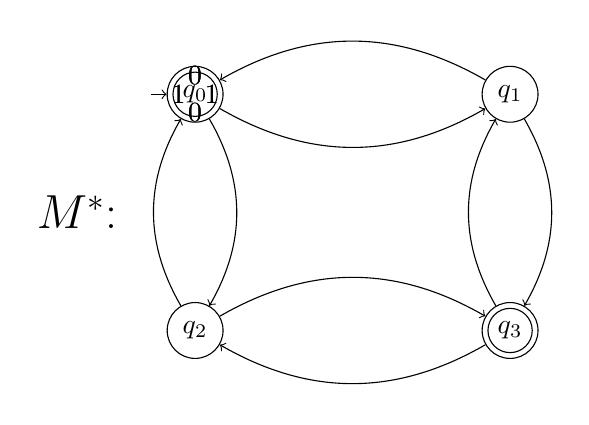
\begin{tikzpicture}[node distance = 3cm]
\node at(-1.5cm,-1.5cm) {\LARGE{$M^*$:}};

\node[circle,draw] (q0) {$q_0$};
\node[circle,draw] (q1) [right of=q0, node distance = 4cm] {$q_1$};
\node[circle,draw] (q2) [below of=q0] {$q_2$};
\node[circle,draw] (q3) [below of=q1] {$q_3$};

\draw[->] (q0.west) +(-0.2,0) -- (q0.west);

\draw[<-] (q0) to [out=30,in=150] (q1) node[above, midway] {$0$};
\draw[->] (q0) to [out=-30,in=-150] (q1) node[below, midway] {$0$};
\draw[->] (q2) to [out=30,in=150] (q3) node[above, midway] {$0$};
\draw[<-] (q2) to [out=-30,in=-150] (q3) node[below, midway] {$0$};

\draw[->] (q0) to [out=-60,in=60] (q2) node[right, midway] {$1$};
\draw[<-] (q0) to [out=-120,in=120] (q2) node[left, midway] {$1$};

\draw[->] (q1) to [out=-60,in=60] (q3) node[right, midway] {$1$};
\draw[<-] (q1) to [out=-120,in=120] (q3) node[left, midway] {$1$};

\draw (q0.center) circle (8pt);
\draw (q3.center) circle (8pt);
\end{tikzpicture}

$M = \rklamm{\gklamm{q_0, q_1, q_2, q_3}, \Sigma_{\tx{Bool}}m, \delta, q_0, \gklamm{q_0, q_3}}$ mit $\delta$:
\begin{table}[htb]
\begin{tabular}{c|c|c}
& $0$ & $1$\\\hline
$q_0$ & $q_1$ & $q_2$\\
$q_1$ & $q_0$ & $q_3$\\
$q_2$ & $q_3$ & $q_0$\\
$q_3$ & $q_2$ & $q_1$
\end{tabular}
\end{table}
\end{beispiel}

\begin{fdefinition}
Sei $M = (Q, \Sigma, \delta, q_0, F)$ ein \ac{DEA}. Eine \indexn{Konfiguration} von $M$ ist ein Paar aus $Q \times \Sigma^*$. $(q_0, w)$ hei�t \indexn{Startkonfiguration} und $(q, \epsilon)$ \indexn{Endkonfiguration} (f�r \ac{bel.} $w \in \Sigma^*$). Gilt f�r eine Endkonfiguration $(q, \epsilon)$ das $q \in F$, so hei�t diese akzeptierend, ansonsten verwerfend. \qed
\Mark{Definition 3.2}
\end{fdefinition}

\begin{fdefinition}
Sei $M = (Q, \Sigma, \delta, q_0, F)$ ein \ac{DEA}. Ein \indexn{Konfigurations�bergang} (ein Schritt) ist eine Relation $\vd_M$: $(Q \times \Sigma^*) \times (Q \times \Sigma^*)$, die \ac{def.} ist durch
\[(p, \underbrace{a}_{\tx{Lesekopf}}\overbrace{w}^{\tx{Band}}) \vd (q, w) \tx{ \ac{gdw.} } \delta(p, a) = q\]

\begin{center}
    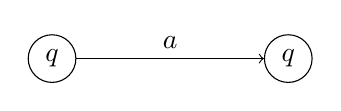
\begin{tikzpicture}[node distance = 3cm]
\node[circle,draw] (nodeone) {$q$};
\node[circle,draw] (nodetwo) [right of=nodeone] {$q$};

\draw[->] (nodeone.east) -- (nodetwo.west) node[above, midway] {$a$};
\end{tikzpicture}
\end{center}

mit $p, q \in Q$, $w \in \Sigma^*$ und $a \in \Sigma$. $\vd_u$ nennen wir \indexn{Schrittrelation}.
\Mark{Definition 3.3}
\end{fdefinition}

\begin{fdefinition}
Sei $M = (Q, \Sigma, \delta, q_0, F)$ ein \ac{DEA} und $w \in \Sigma^*$. Eine Berechnung $c$ von $M$ ist eine endliche Folge von Konfigurationen
\[c = c_0, \dots, c_n \tx{ mit } c_i \vd c_{i + 1} (1 \klgl i \klgl n - 1)\]
$c$ ist eine Berechnung von $M$ f�r eine Eingabe $w$, falls $c_0 = (q_0, w)$ (Startkonfiguration) und $c_n = (q, \epsilon)$ (Endkonfiguration). Falls $c_n$ \ac{akzept.} Endkonfiguration ist, so ist C \ac{akzept.} Berechnung; ansonsten verwerfende Berechnung.
\Mark{Definition 3.4}
\end{fdefinition}

\begin{beispiel}
\[(q_0, \underline{1}001) \vd (q_2, 001) \vd (q_3, 01) \vd (q_2, 1) \vd (\underbrace{q_0}_{\in F}, \epsilon)\]
ist \ac{akzept.} Berechnung von $M^*$ (zu GI(V)-15.04.2009-DIA-1) auf $1001$
\end{beispiel}

\begin{fdefinition}
Sei $M = (Q, \Sigma, \delta, q_0, F)$ ein \ac{DEA}. Wir definieren: $\vd_M^*$: $(Q \times \Sigma^*) \times (Q \times \Sigma^*)$ als reflexiven und transitiven Abschluss von $\vd$:
\begin{itemize}
\item $(q, w) \vd^* (q, w)$ $\forall q \in Q, w \in \Sigma^*$
\item $(p, uv) \vd^* (q, v)$, falls $u = a_1 \dots a_n (a_i \in \Sigma)$ $\exists q_1, \dots, q_{n - 1} \in Q$, so dass
		\[(p, a_1 \dots a_n v) \vd (q_1, a_1 \dots a_n v) \vd \dots \vd (q_{n - 1}, a_n v) \vd (q, v)\]
		f�r $p, q \in Q$ $u, v \in \Sigma^*$
\end{itemize}
Die Fortsetzung $\hat{\delta}$: $Q \times \Sigma^* \ra Q$ der Transitionsfunktion $\delta$ auf W�rter \ac{def.} wir induktiv durch
\begin{itemize}
\item $\hat{\delta} (q, \epsilon) = q$
\item $\hat{\delta} (q, wa) = \delta(\hat{\delta} (q, w))$ $\forall w \in \Sigma^*$, $a \in \Sigma$ und $q \in Q$
\end{itemize}
\Mark{Definition 3.5}
\end{fdefinition}

\begin{fnotation}
Falls $\hat{\delta} (q, w) = p$, so schreiben wir
\[q \stack{w}{\longrightarrow} p\]
und sagen es existiert ein Pfad von $q$ nach $p$ mit Beschriftung $w$.
\end{fnotation}

\begin{fdefinition}
Sei $M = (Q, \Sigma, \delta, q_0, F)$ ein \ac{DEA}. Die von $M$ akzeptierte Sprache $L(M)$ ergibt sich aus:
\begin{align*}
L(M) &= \gklamm{w \in \Sigma^* \vert \hat{\delta}(q_0, w) \in F}\\
&= \gklamm{w \in \Sigma^* \vert q_0 \stack{w}{\longrightarrow} q \tx{ und } q \in F}\\
&= \gklamm{w \in \Sigma^* \vert (q_0, w) \vd^* (q, \epsilon) \tx{ mit } q \in F}
\end{align*}
Sprachen, die von einem \ac{DEA} erkannt werden nennt man regul�re Sprachen. Zwei \ac{DEA}s $M_1$ und $M_2$ sind �quivalent \ac{gdw.} $L(M_1) = L(M_2)$
\Mark{Definition 3.6}
\end{fdefinition}

\begin{lemma}
Der \ac{DEA} $M_x = \rklamm{\Sigma_{\tx{Bool}}, Q, \delta, q_0, F}$ erkennt die Sprache
\[L(M_x) = \gklamm{w \in \Sigma_{\tx{Bool}}^* \vert \rklamm{\betrag{w}_0 + \betrag{w}_1} \mod 2 = 0}\]
\end{lemma}

\begin{fbeweis}
F�r jedes Wort $w \in \Sigma_{\tx{Bool}}^*$ bleibt der Automat $M_x$ in einem bestimmten Zustand stehen. Betrachten wir f�r einen \ac{bel.} Zustand die Menge der W�rter, f�r die $M_x$ in exakt diesem Zustand terminiert.
\[\mathcal{K} (q) = \gklamm{w \in \Sigma_{\tx{Bool}}^*\vert q_0 \stack{w}{\longrightarrow} q}\]
Da $M_x$ deterministisch ist, kann ein Wort, welches in $\mathcal{K}(q)$ liegt nicht gleichzeitig in $\mathcal{K}\rklamm{q^{\frownie}}$ liegen (mit $q \neq q^{\frownie}$) - $\mathcal{K}(q) \cap \mathcal{K}\rklamm{q^{\frownie}} = \emptyset$. Die Menge der von $M_x$ erkannten W�rter entspricht der Vereinigung aller Mengen $\mathcal{K}(q)$, die sich auf akzeptierende Zust�nde beziehen.
\[L(M_x) = \bigcup_{q \in F} \mathcal{K}(q)\]
$\mathcal{K}$ ist eine �quivalenzklasse folgender Relation $R_s$
\begin{align*}
&u R_{\delta} v = \hat{\delta} (q_0, u) = \hat{\delta} (q_0, u)\\
&R_{\delta} (w, v)
\end{align*}
in $\mathcal{K} (q)$ befindet sich nur solche W�rter, die \ac{bzgl.} $R_{\delta}$ in Relation stehen.

Beweisidee:
\begin{itemize}[label=-]
\item Ordne $q_i (0 \klgl i \klgl 3)$ konkrete �quivalenz-Klassen zu \textcircled{$\star$}
\item Zeige $\mathcal{K} (q_0) \cup \mathcal{K} (q_3) = L(u)$
\item Zeige, dass \textcircled{$\star$} korrekt.
\end{itemize}
\Solved{�ndere \textcircled{*} in ein sch�neres Symbol}{Replaced with \textcircled{$\star$}}
Wir stellen folgende Induktionsannahme auf:
\begin{align*}
&\mathcal{K} (q_0) = \gklamm{w \in \Sigma_{\tx{Bool}}^*~\vert~\betrag{w}_0 \tx{ und } \betrag{w}_1 \tx{ sind gerade}}\\
&\mathcal{K} (q_1) = \gklamm{w \in \Sigma_{\tx{Bool}}^*~\vert~\betrag{w}_0 \tx{ ungerade } \vert \betrag{w}_1 \tx{ gerade}}\\
&\mathcal{K} (q_2) = \gklamm{w \in \Sigma_{\tx{Bool}}^*~\vert~\betrag{w}_0 \tx{ gerade } \vert \betrag{w}_1 \tx{ ungerade}}\\
&\mathcal{K} (q_3) = \gklamm{w \in \Sigma_{\tx{Bool}}^*~\vert~\betrag{w}_0 \tx{ und } \betrag{w}_1 \tx{ ungerade}}
\end{align*}

\begin{enumerate}
\item Induktionsanfang: wir zeigen, dass $\vert A$ f�r W�rter der L�nge $\klgl 2$ gilt
		\begin{align*}
		0:~~&\delta \rklamm{q_0, \epsilon} = q_0 \Ra \epsilon \in \mathcal{K}(q_0) \checkmark\\
		1:~~&\delta (q_0, 1) = q_2, 1 \in \mathcal{K}(q_2) \checkmark\\
			&\delta (q_0, 0) = q_1, 0 \in \mathcal{K}(q_1) \checkmark\\
		2:~~&\hat{\delta} (q_0, 00) = q_0, 00 \in \mathcal{K} (q_0) \checkmark\\
			&\hat{\delta} (q_0, 01) = q_3, 01 \in \mathcal{K} (q_3) \checkmark\\
			&\hat{\delta} (q_0, 10) = q_3, 10 \in \mathcal{K} (q_3) \checkmark\\
			&\hat{\delta} (q_0, 11) = q_0, 11 \in \mathcal{K} (q_0) \checkmark
		\end{align*}
\item Induktionsschluss: Wir setzen voraus, dass der Induktionsanfang f�r W�rter $\betrag{u} \klgl i$ gilt. Wir wollen jetzt zeigen, dass der Induktionsanfang dann auch f�r W�rter der L�nge $i + 1$ gilt.\\
		Sei also $w \in \Sigma_{\tx{Bool}}^{i + 1}$, also $w = u \mal a$ mit $u \in \Sigma_{\tx{Bool}}^{i}$ und $a \in \Sigma_{\tx{Bool}}$. Wir m�ssen vier F�lle unterscheiden:
		\begin{enumerate}[label=\arabic*.]
		\item $\betrag{u}_0$ gerade, $\betrag{u}_1$ gerade. Laut Induktionsvoraussetzung gilt $\hat{\delta} (q_0, u) = q_0$ \ac{bzw.} $u \in \mathcal{K} (q_0)$. Wir erhalten
				\[\hat{\delta} (q_0, ua) = \delta \rklamm{\hat{\delta} (q_0, u), a} \stack{\tx{IV}}{=} \delta(q_0, a) = \begin{cases}q_1 \tx{ falls } a = 0\\q_2 \tx{ falls } a = 1\end{cases}\]
				Da $\betrag{u1}_0$ gerade und $\betrag{u1}_1$ ungerade entspricht $\hat{\delta} (q_0, u1) = q_2$ der IA.\\
				Da $\betrag{u0}_0$ ungerade und $\betrag{u0}_1$ gerade entspricht $\hat{\delta} (q_0, u0) = q_1$ der IA.
		\item analog, trivial, selbst! 
		\item analog, trivial, selbst!
		\item analog, trivial, selbst!
		\end{enumerate}
\end{enumerate}
\end{fbeweis}

\section{Nichtdeterministische endliche Automaten (NEAs)}
\Mark{Section 3.3}
\Insert{IMG-GI-09-04-21-1}
\begin{fdefinition}
Ein \ac{NEA} $M$ ist ein Quintupel $(Q, \Sigma, \delta, q_0, F)$ aus
\begin{itemize}
\item $Q, \Sigma, q_0, F$ wie \ac{DEA}
\item eine Transitionsfunktion $\delta$: $Q \times \Sigma \ra \mathcal{P} (Q)$
\end{itemize}
\end{fdefinition}

\begin{fnotation}
Falls $q \in \delta(p, a)$ schreiben wir $p \stack{a}{\ra} q$
\end{fnotation}
